\documentclass{beamer}

%-----------------------------------------Packages---------------------------------

\usepackage[cm-default]{fontspec}
\usepackage{xunicode}
\usepackage{amsmath}
\usepackage{amssymb}
\usepackage{mathrsfs}
\usepackage{fontspec} %加這個就可以設定字體
\usepackage{multirow}
%\usepackage{xeCJK} % 讓中英文字體分開設置

\usepackage{xltxtra}
\usepackage{latexsym}
\usepackage{amsmath}
\usepackage{amssymb}
\usepackage{mathrsfs}
\usepackage{booktabs}
\usepackage{bm} %公式粗体
\usepackage{multirow}
\usepackage{graphicx}
\usepackage{indentfirst}
\usepackage{fancyhdr} %页眉页脚
\usepackage{listings}
\usepackage{color}
\usepackage{hyperref}



%\setsansfont[Mapping=tex-text]{WenQuanYi Micro Hei} %设置中文字体
%\XeTeXlinebreaklocale "zh" %设置换行格式
%\XeTeXlinebreakskip = 0pt plus 1pt %這兩行一定要加,中文才能自動換行

\usetheme{Darmstadt}


%插入代码段
\definecolor{mygreen}{rgb}{0,0.6,0}
\definecolor{mygray}{rgb}{0.5,0.5,0.5}
\definecolor{mymauve}{rgb}{0.58,0,0.82}

\lstset{ %
  backgroundcolor=\color{white},   % choose the background color; you must add \usepackage{color} or \usepackage{xcolor}
  basicstyle=\footnotesize,        % the size of the fonts that are used for the code
  breakatwhitespace=false,         % sets if automatic breaks should only happen at whitespace
  breaklines=true,                 % sets automatic line breaking
  captionpos=b,                    % sets the caption-position to bottom
  commentstyle=\color{mygreen},    % comment style
  deletekeywords={...},            % if you want to delete keywords from the given language
  escapeinside={\%*}{*)},          % if you want to add LaTeX within your code
  extendedchars=true,              % lets you use non-ASCII characters; for 8-bits encodings only, does not work with UTF-8
  frame=single,                    % adds a frame around the code
  keepspaces=true,                 % keeps spaces in text, useful for keeping indentation of code (possibly needs columns=flexible)
  keywordstyle=\color{blue},       % keyword style
  language=Octave,                 % the language of the code
  morekeywords={*,...},            % if you want to add more keywords to the set
  numbers=left,                    % where to put the line-numbers; possible values are (none, left, right)
  numbersep=5pt,                   % how far the line-numbers are from the code
  numberstyle=\tiny\color{mygray}, % the style that is used for the line-numbers
  rulecolor=\color{black},         % if not set, the frame-color may be changed on line-breaks within not-black text (e.g. comments (green here))
  showspaces=false,                % show spaces everywhere adding particular underscores; it overrides 'showstringspaces'
  showstringspaces=false,          % underline spaces within strings only
  showtabs=false,                  % show tabs within strings adding particular underscores
  stepnumber=2,                    % the step between two line-numbers. If it's 1, each line will be numbered
  stringstyle=\color{mymauve},     % string literal style
  tabsize=2,                       % sets default tabsize to 2 spaces
  title=\lstname                   % show the filename of files included with \lstinputlisting; also try caption instead of title
}

\lstdefinestyle{custombash}{
    language=bash,
    morekeywords={*,compact,similarity,predict}
}

%-----------------------------------------Funcions-------------------------------------------
%章节首突出显示目录
\AtBeginSection[]  %每个section前突出Section的各Sub
{
    \begin{frame}<beamer>{Content}
          \tableofcontents[currentsection]
     \end{frame}
}

\AtBeginSubsection[]  %每个subsection前突出该Sub与其所在Section
{
    \begin{frame}<beamer>{Content}
          \tableofcontents[currentsection,currentsubsection]
     \end{frame}
}
\begin{document}

%-----------------------------------------Title-------------------------------------------
\title{Collaborative Filtering Implementation and Evaluation}
\subtitle{Recommender System for Ecommerce Data}
\author[Harttle]{Jun Yang}
\institute[PKU]{
  School of Electronic and Computer Engineering, Peking University
}
\date{\today}

%Title Page
\begin{frame}[plain]
  \titlepage
\end{frame}

%Overview
\begin{frame}<beamer>{Overview}
	\tableofcontents
\end{frame}

%------------------------------------------Body----------------------------------------------

\section{Introduction}

\subsection{Recommender System}

\begin{frame}[fragile]
	\frametitle{What is Recommender System?}

    Identify a set of items that will be of interest to a certain user.

    \begin{columns}
        \column{.5\textwidth}

        \begin{itemize}
        \item Similarity between items/users will be analyzed.
        \item Historical data will be used.
        \end{itemize}

        \column{.5\textwidth}

            \begin{block}{\$1,000,000 Prize}
                
\includegraphics[width=\linewidth]{./netflix.png}
            \end{block}

    \end{columns}

\end{frame}

\begin{frame}[fragile]{Classes of Recommeder System}
	\begin{itemize}
        \item Collaborative Filtering (CF)
        \begin{itemize}
        \item User-based: Facebook, LinkedIn
        \item Item-based: Amazon
        \end{itemize}

        \item Content-based
        \begin{itemize}
        \item Information-Retrieval: tf-idf, LSM
        \item Machine-Learning: clusters, classifiers, neural networks
        \end{itemize}
	\end{itemize}
\end{frame}

\subsection{Collaborative Filtering}

\begin{frame}[fragile]{User-based Collaborative Filtering}

\begin{enumerate}
\item Identify a neighborhood of people with similar behavior.
\item Analyze this neighborhood to find out recommends.
\end{enumerate}

\begin{equation}
P_{u,i} = \sum_{Rank(s_{u,v})>k}s_{u,v} \cdot R_{v,i}
\end{equation}

\end{frame}

\begin{frame}[fragile]{Problems with User-based CF}

\begin{block}{Sparsity}
        Limited information for a certain user caused inaccuracy when identifying neiborhood, thus poor recommendations.
        \end{block}
\begin{block}{Scalability}
        Computation grows linearly with the number of users.
        \end{block}

\begin{block}{New User Problem}
        We have nothing to recommend to new users.
        \end{block}

\end{frame}

\begin{frame}[fragile]{Item-based Collaborative Filtering}

\begin{enumerate}
\item Identify a neighborhood of items.
\item Analyze this neighborhood to find out recommends.
\end{enumerate}

\begin{equation}
P_{u,i} = \sum_{Rank(s_{i,j})>k}s_{i,j} \cdot R_{u,j}
\end{equation}

\end{frame}

\section{Item-based Collaborative Filtering}

\begin{frame}{Terminology}

\begin{itemize}
\item Users $U$\\
        The collection of users.
\item Items $I$\\
        The collection of items.
\item Rating $R$\\
        $R_{i,j}$ represents user $i$'s rating for item $j$.
\item Similarity $S$\\
        $S_{i,j}$ represents the similarity between user/item $i$ and $j$.
\item Prediction $P$ \\
        $P_{i,j}$ represents user $i$'s predicted rating for item $j$.
\end{itemize}

\end{frame}

\begin{frame}[allowframebreaks]{Algorithm}

\begin{enumerate}
\item Get input ratings: $R$
\item Compute similarities: $S$
    \begin{equation}
        S_{i,j} = sim(\vec{R_i},\vec{R_j})
    \end{equation}
    where: \\
    $\vec{R_i} = (R_{1,i},R_{2,i},\cdots,R_{N,i})$\\
    $\vec{R_j} = (R_{1,j},R_{2,j},\cdots,R_{N,j})$
\item Identify $k$ neighbors $\{j_1,j_2,\cdots,j_k\}$ for each item.

\newpage

\item For each user who bought a set of items $C$:
    \begin{enumerate}
    \item Neighbors of $c \in C$ forms candidates: $N$, remove $n \in N$ that is already in $C$.
    \item For each $n \in N$, compute its similarity with $C$ as the sum of similarities with $c \in C$.
    \item Sort $N$ respect to that similarities.
    \end{enumerate}
\item The sorted $N$ for each user forms recommendation set.
\end{enumerate}

\end{frame}

\section{Implementation}

\subsection{Rating}

\begin{frame}[fragile]{Data Format}

\begin{itemize}
\item Formart:

\begin{lstlisting}
#user_id    item_id type    date
847750      2235    0       4.15
847750      2215    1       4.16
6694750     14020   0       6.16
\end{lstlisting}
\item Statistic:

\begin{table}[!h]
\centering
%\caption{Page Rank }
\begin{tabular}{|l|l|}
\hline
No. Users & 860 \\ \hline
No. Items & 7842 \\ \hline
No. Lines & 42531 \\ \hline
Begin Date & 15th, April\\ \hline
End Date & 15th, August\\ \hline
\end{tabular}
\end{table}

\end{itemize}

\end{frame}


\begin{frame}{Behavior Statistics}

Ratings matrix $R$ is required to do collaborative filtering, how to get $R$ from the dataset?

\begin{itemize}
\item If user $u$ bought item $i$, then $R_{u,i}$ = 1.
\end{itemize}

\begin{alertblock}{What about user $u$ clicked item $i$ ?}
\begin{itemize}
\item When a user clicked an item, it's likely that he'll buy it. As time goes, the probability buy decreases.
\item Make statistics about probability with respective to time:

    \begin{equation}
    p = f(t)
    \end{equation}

\item The rating:
    \begin{equation}
    R_{u,i} = \int_{prediction~timespan}f(t)dt
    \end{equation}

\end{itemize}
\end{alertblock}

\end{frame}

\begin{frame}{Integrated Probability for Click Behavior}
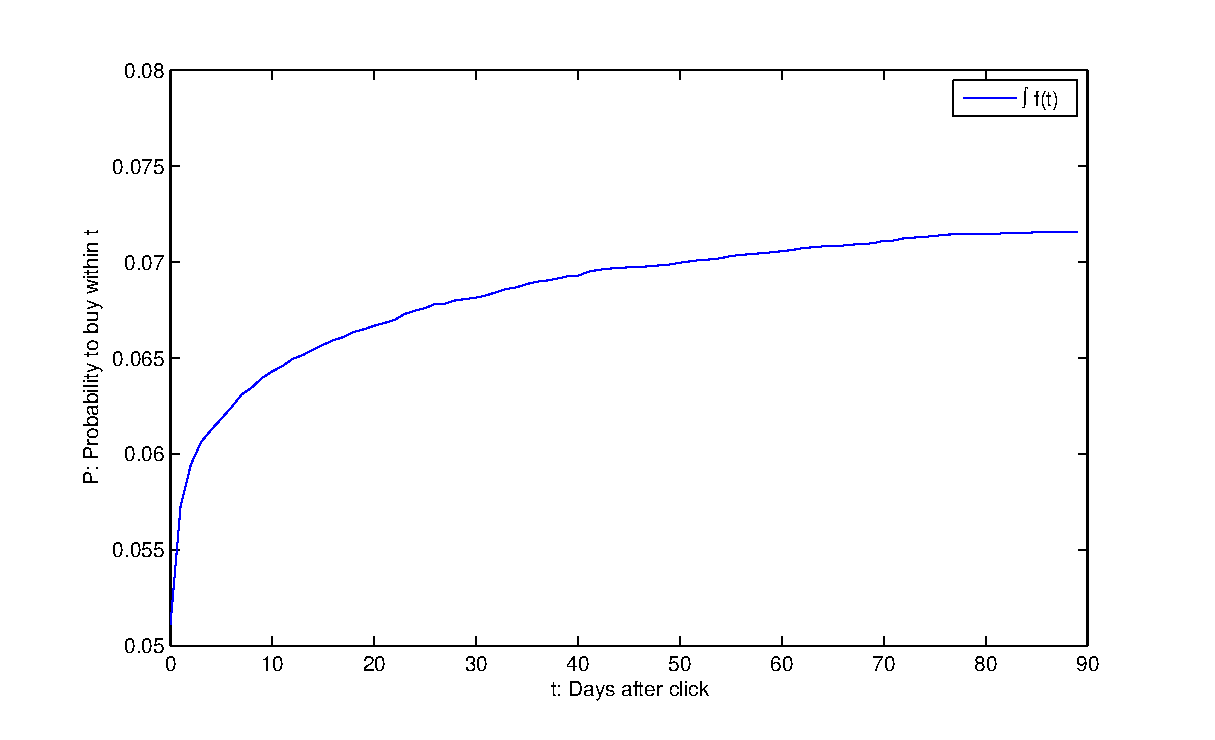
\includegraphics[width=\linewidth]{./click_curve.eps}
\end{frame}

\subsection{Item Similarity}

\begin{frame}{Similarity Methods}

Similarity between items are usually computed in the space of $users$, treating each item as a vector. Classes of similarity methods:

\begin{itemize}
\item Cosine similarity
\item Adjusted cosine similarity
\item Pearson Correlation coefficient
\end{itemize}

\end{frame}


\begin{frame}{Cosine Similarity}

\begin{equation}
sim(\vec{u},\vec{v}) = \cos(\vec{u},\vec{v}) = \frac{\vec{u}\cdot \vec{v}}{||\vec{u}|| \cdot ||\vec{v}||}
\end{equation}

\begin{itemize}
\item Similarity tends to be high when if each user who purchases u also purchases v as well.
\item Frequently purchased items are de-emphasized by the denominator.
\item The result range: $[0,1]$
\end{itemize}


\end{frame}

\begin{frame}{Adjusted Similarity}

\begin{equation}
sim(i,j) = \frac{\sum_{u \in U}(R_{u,i} - \overline{R_u})(R_{u,j} - \overline{R_u})}{\sqrt{\sum_{u \in U}(R_{u,i} - \overline{R_u})^2}\sqrt{\sum_{u \in U}(R_{u,j} - \overline{R_u})^2}}
\end{equation}

\begin{itemize}
\item Different rating scales between users are taken into account.
\item The result range: $[-1,1]$
\end{itemize}

\end{frame}


\begin{frame}{Pearson Correlation Coefficient}

\begin{equation}
sim(i,j) = \frac{\sum_{u \in U}(R_{u,i} - \overline{R_i})(R_{u,j} - \overline{R_j})}{\sqrt{\sum_{u \in U}(R_{u,i} - \overline{R_i})^2}\sqrt{\sum_{u \in U}(R_{u,j} - \overline{R_j})^2}}
\end{equation}

\begin{itemize}
\item $Pearson-r$ is a measure of the linear dependence between two variables.
\item We need isolate co-rated cases in advance.
\item The result range: $[-1,1]$
\end{itemize}

\end{frame}


\subsection{Prediction}


\begin{frame}{Similarity Summing}

As mentioned above, $P_{u,i}$ is computed by summing the similarities between item $i$ and items in user $u$'s basket:

\begin{equation}
P_{u,i} = \sum_{Rank(s_{i,j})>k} s_{i,j} \cdot R_{u,j}
\end{equation}

\begin{block}{Better summing method?}
\begin{itemize}
\item Treat recommendations from each item $j$ as independent events.
\item Only when all recommendation fails, $R_{u,i} = 0$. Thus:

\begin{equation}
P_{u,i} = 1 - \prod_{Rank(s_{i,j})>k} (1 - s_{i,j} \cdot R_{u,j})
\end{equation}
\end{itemize}
\end{block}

\end{frame}


\begin{frame}{Similarity Normalization}

Yet our summing method don't take into account the difference in density of the $k$ neighbors.

\begin{equation}
P_{u,i} = \sum_{Rank(s_{i,j})>k} s_{i,j} \cdot R_{u,j}
\end{equation}

We can normalize the k similarities so that they add-up to 1.

\begin{exampleblock}{Problem Case}
An infrequently purchased item $i$ have a moderate overlap with another infrequently purchased item $j$, this will cause high similarity and lead to wrong recommendation.
\end{exampleblock}

\end{frame}


\begin{frame}{Row Normalization}

For users who purchases a lot, each item reflects his appetite less. We'll normalize $R$ before doing prediction.

\end{frame}


\begin{frame}{Post Procession}

\begin{itemize}
\item If user $u$ once purchased item $i$, whether he'll purchase another depends on the lifetime of item $i$.
\item Lifetime of item $i$:

    \begin{equation}
    \tau_i \approx \frac{\sum_{u \in U, R_{u,i}=1} R_{u,i}}{\sum_{u \in U, R_{u,i}=1}1 \cdot TimeSpan}
    \end{equation}

\item Thus the modified $R_{u,i}$ will be:

    \begin{equation}
        R'_{u,i} = \left\{ 
        \begin{array}{l l}
        R_{u,i} & \quad \text{if $R_{u,i} \neq 1$ }\\
        \frac{Timespan_{prediction}}{\tau_i} \cdot R_{u,i} & \quad \text{otherwise}
        \end{array} \right.
    \end{equation}

\end{itemize}

\end{frame}

\section{Evaluation}


\begin{frame}{Quality Measure}

The quality of recommender system is measured by $recall$ and $precision$.

\begin{itemize}
\item $recall$ is the percentage of hits in the test set.
\item $precision$ is the percentage of hits in the prediction set.
\item $F1$ is used to combine these two parameters:
    \begin{equation}
    F1 = \frac{2}{1/recall + 1/precision}
    \end{equation}
\end{itemize}

\end{frame}



\begin{frame}{Train Set \& Test Set}

In order to measure recommendation quality, we split the dataset into train set and test set:

\begin{center}
  \begin{tabular}{ | l | l | l | }
    \hline
    ~           & Train Set & Test Set \\ \hline
    Begin Date  & 15th April    & 15th July  \\ \hline
    End Date    & 14th July     & 14th August  \\ \hline
    No. Transaction    & 4971   & 2013    \\ \hline
  \end{tabular}
\end{center}

\end{frame}



\subsection{Effect of Pre and Post Processing}

\begin{frame}{Effect of Pre-processing}
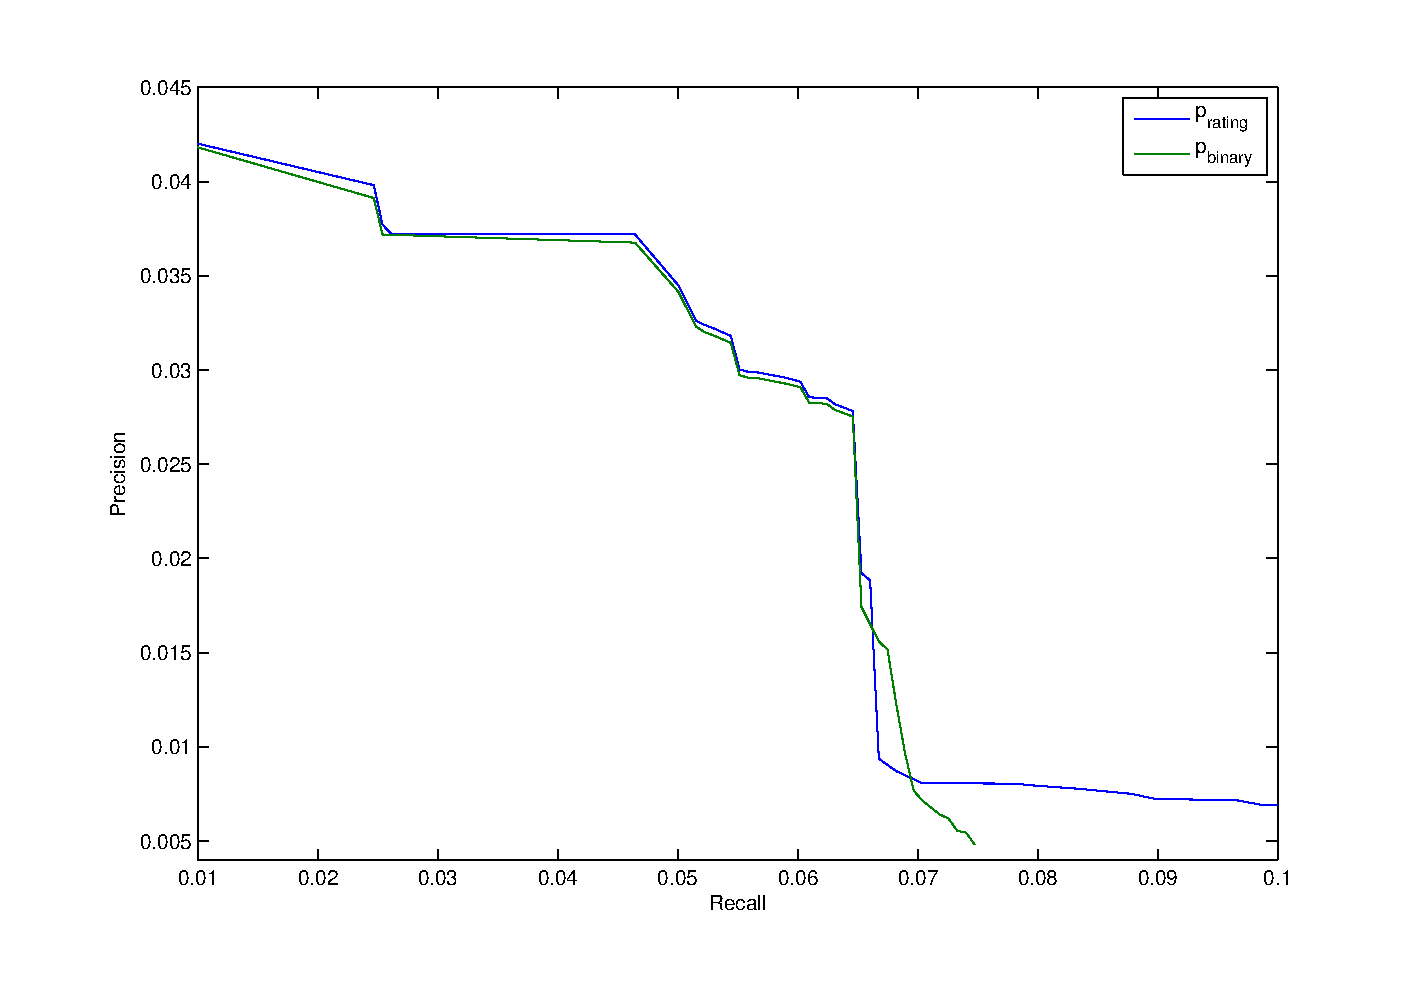
\includegraphics[width=\linewidth]{./rating.eps}
\end{frame}

\begin{frame}{Effect of Pre-processing}
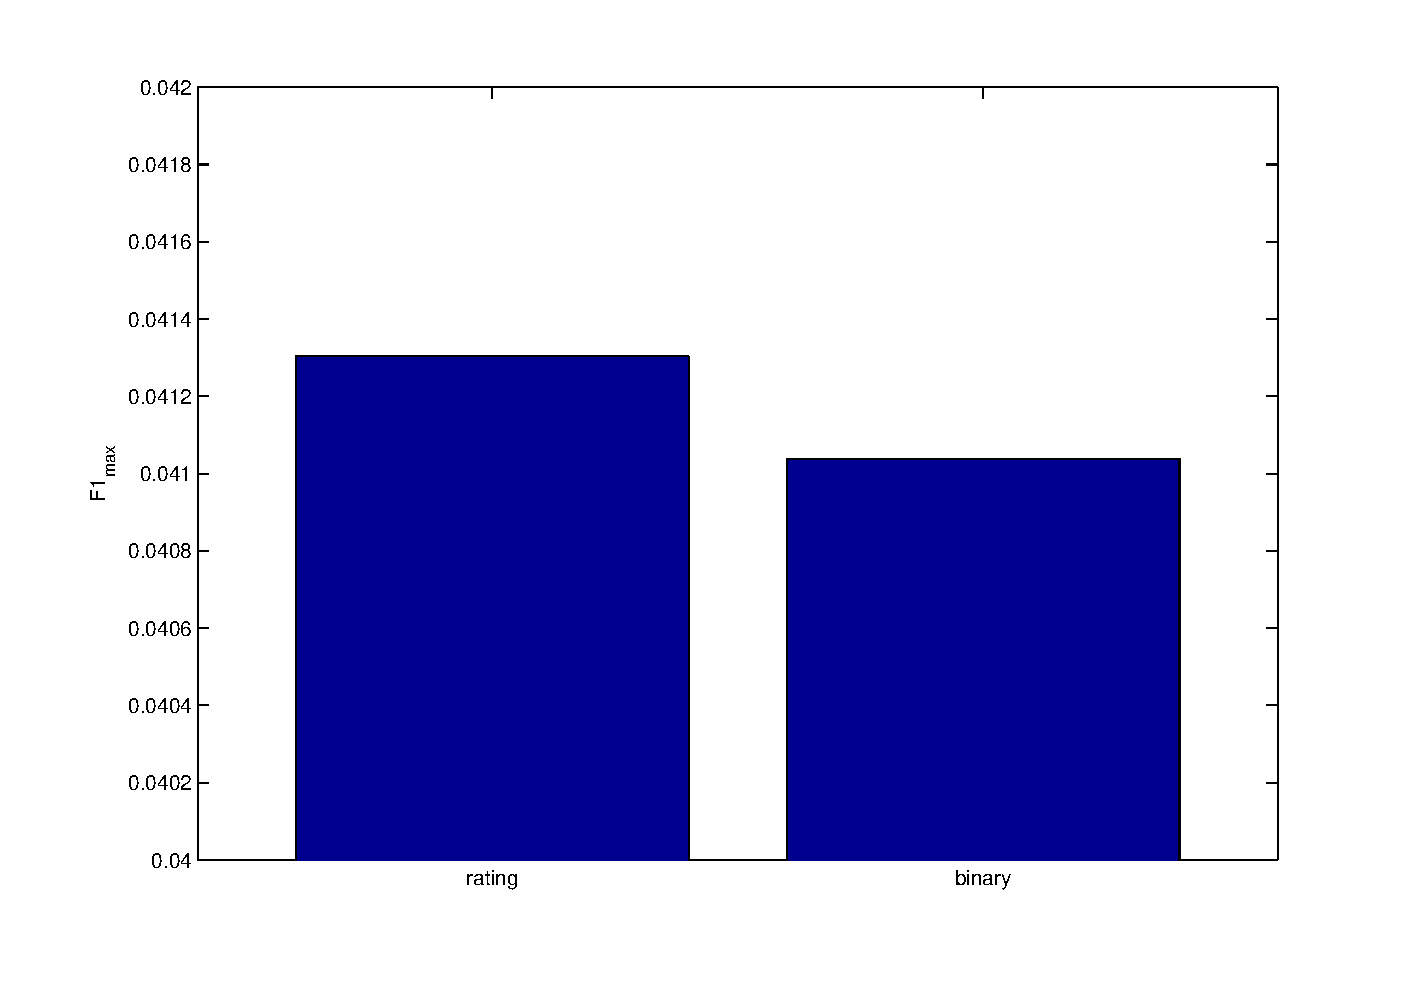
\includegraphics[width=\linewidth]{./rating_f1.eps}
\end{frame}


\begin{frame}{Effect of Post-processing}
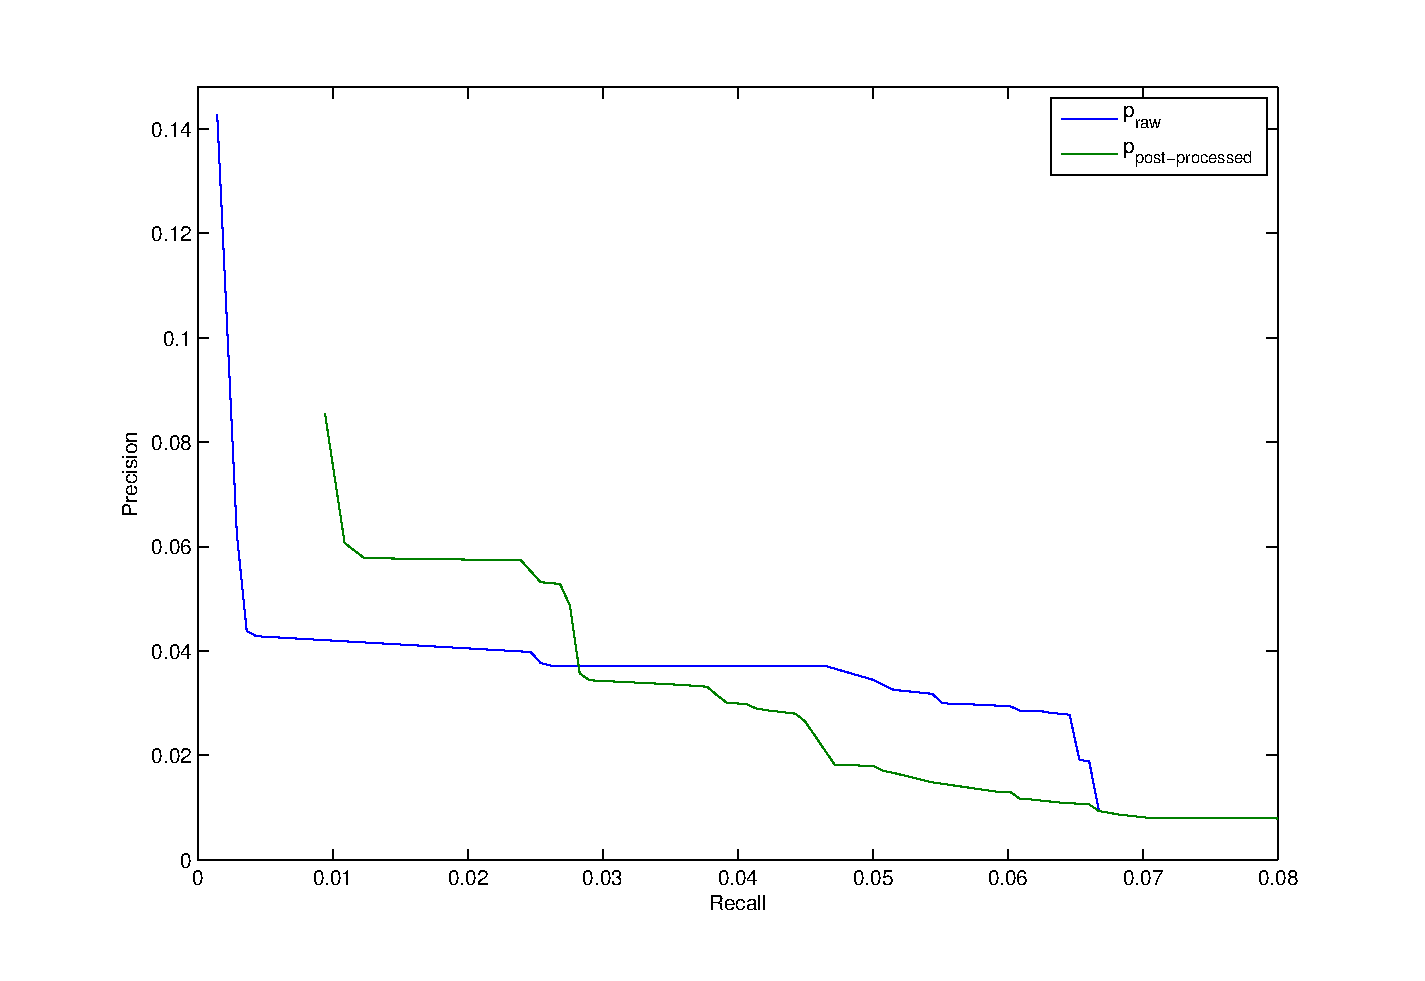
\includegraphics[width=\linewidth]{./post-proc.eps}
\end{frame}

\begin{frame}{Effect of Post-processing}
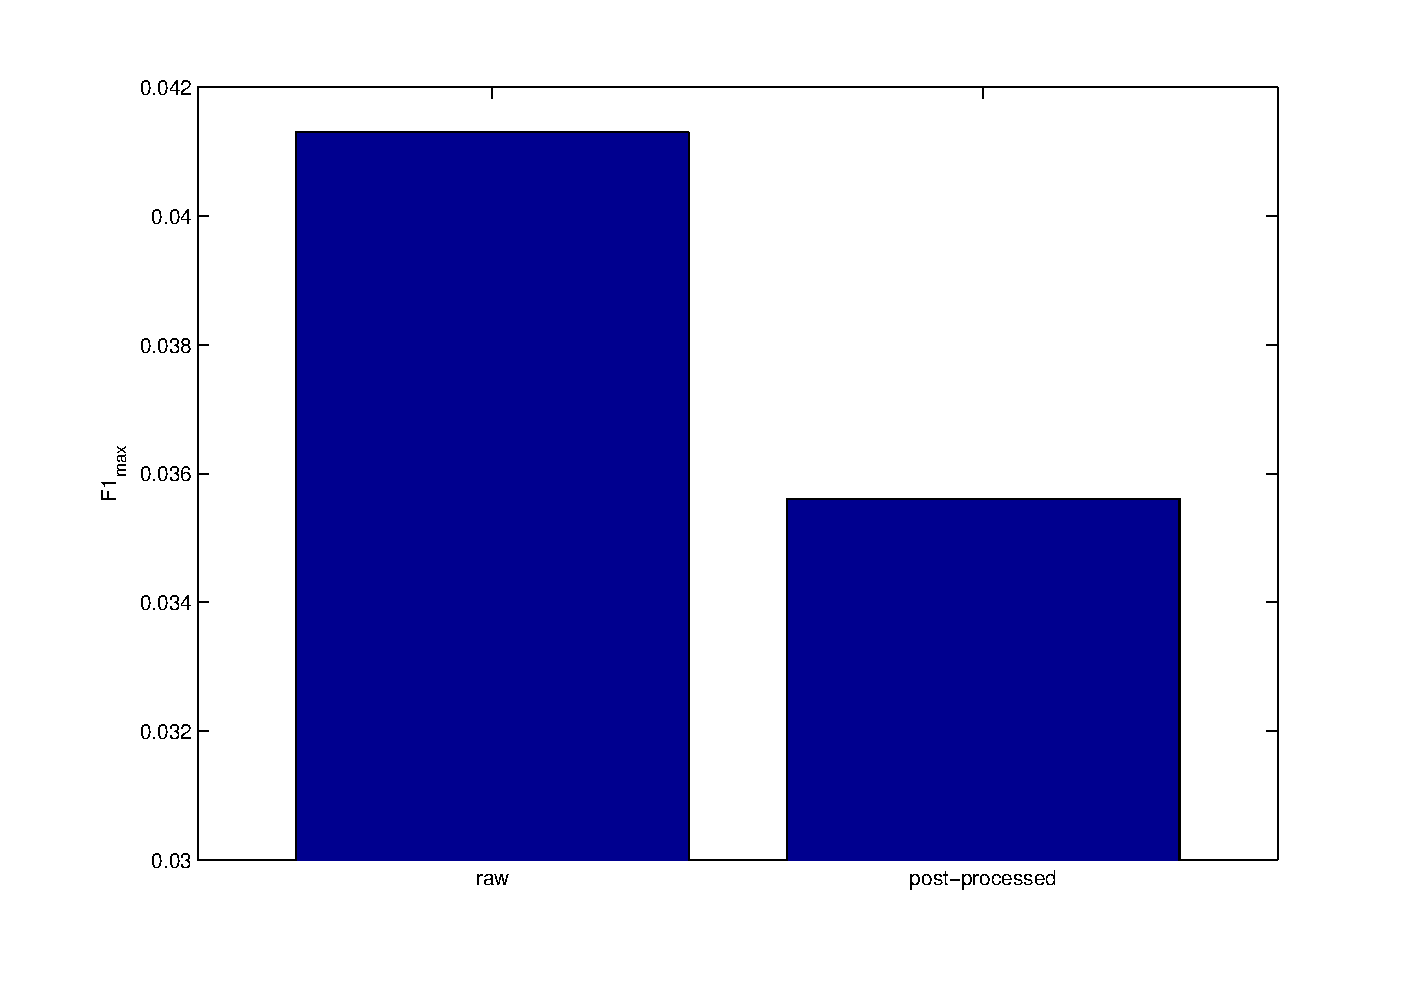
\includegraphics[width=\linewidth]{./post-proc_f1.eps}
\end{frame}



\subsection{Similarity Method Comparison}

\begin{frame}{Similarity Method Comparison}
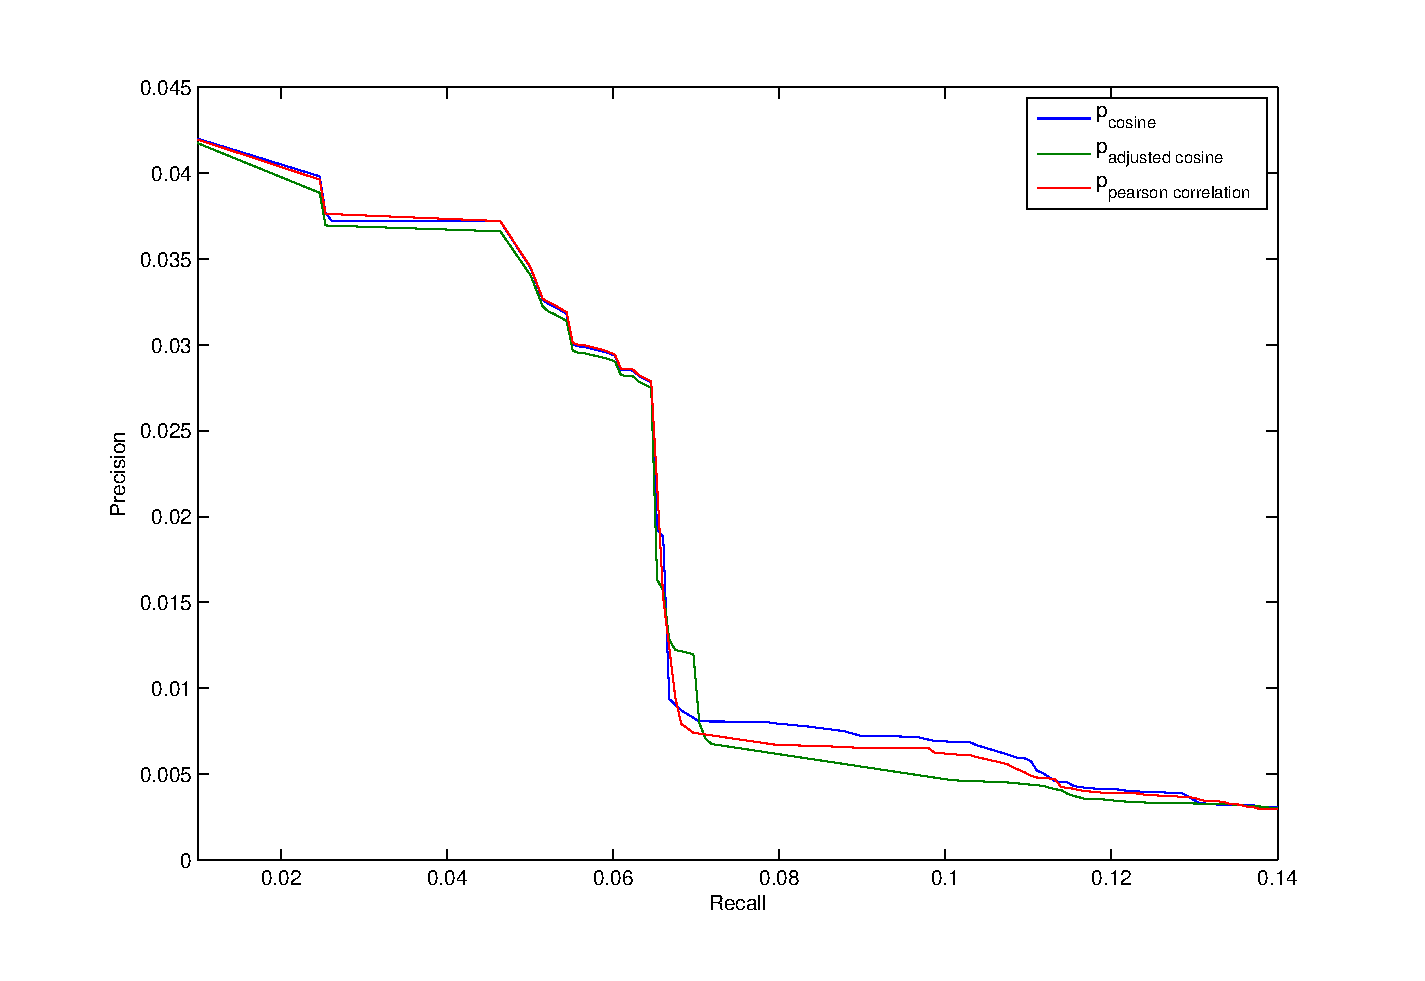
\includegraphics[width=\linewidth]{./sim_compare.eps}
\end{frame}

\begin{frame}{Similarity Method Comparison}
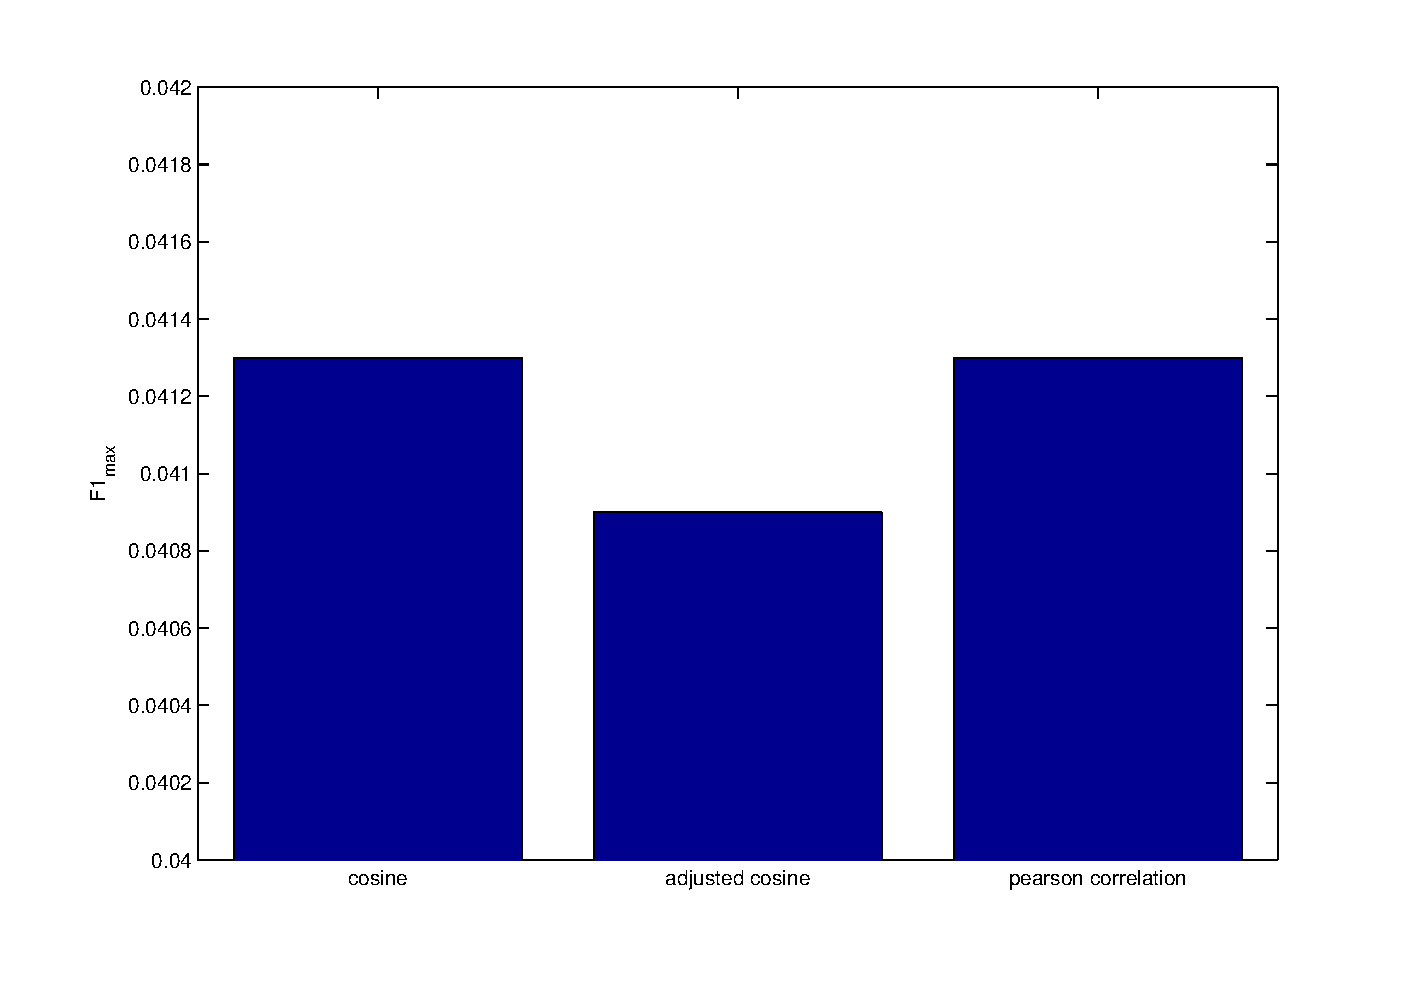
\includegraphics[width=\linewidth]{./sim_compare_f1.eps}
\end{frame}


\begin{frame}{Similarity Method Comparison}

\begin{itemize}
\item Correlation and Cosine are approximate.
\item Adjusted cosine is bad.
\end{itemize}

\begin{exampleblock}{Why adjusted cosine not suitable?}
Adjusted cosine removes the difference in rating scales, which means positive rating could contain negative information.

While for ecommerce data, positive rating is always positive.
\end{exampleblock}

\end{frame}



\subsection{Summing and Normalization}

\begin{frame}{Effect of Similarity Summing Method}
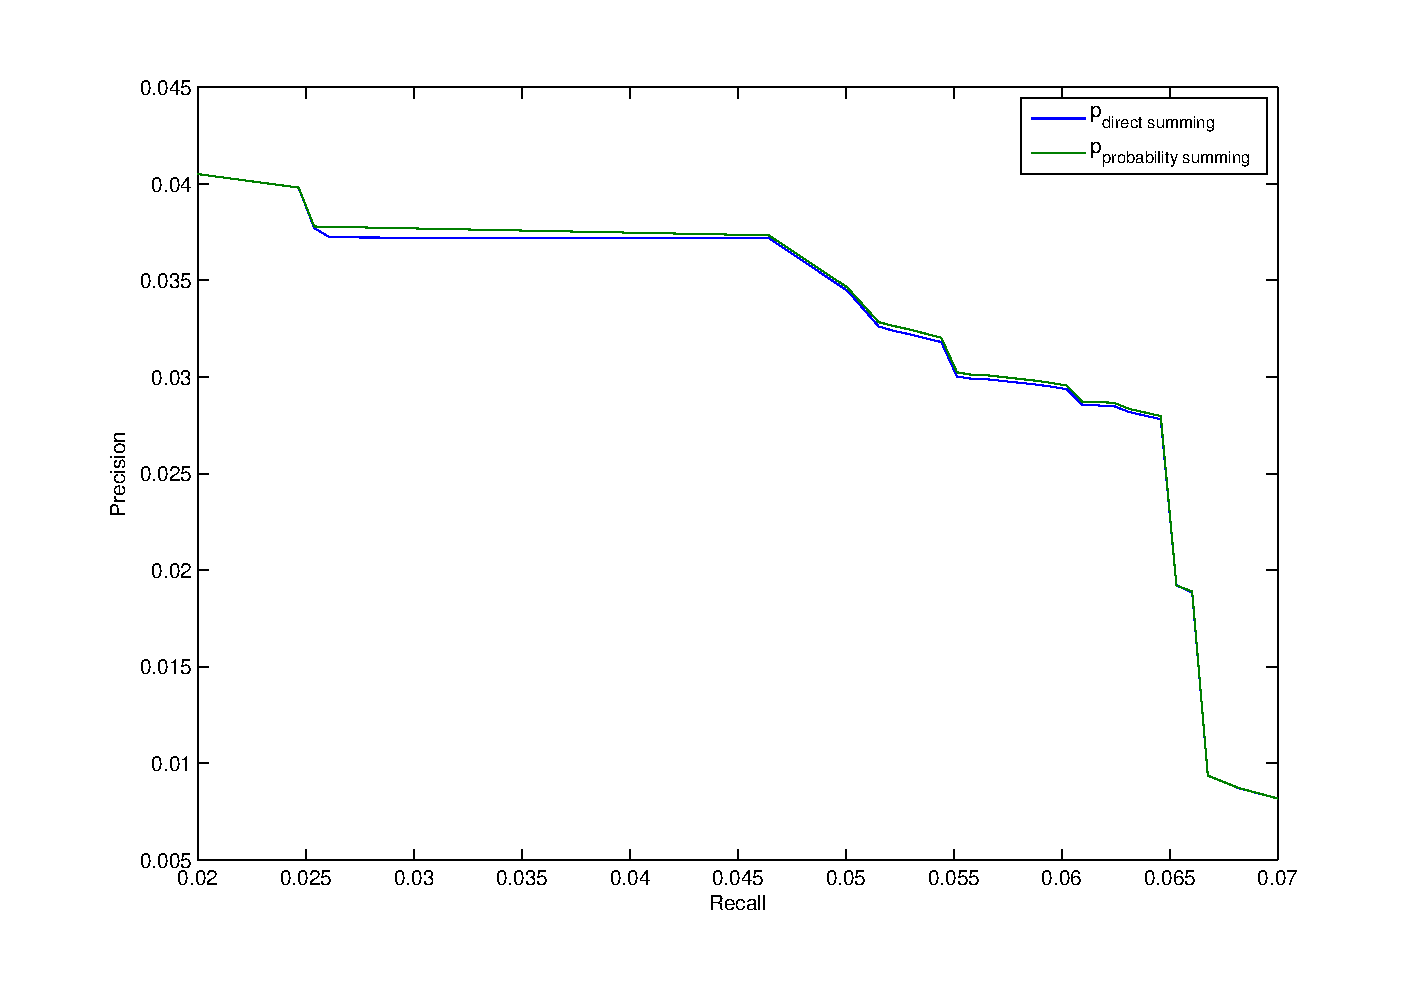
\includegraphics[width=\linewidth]{./summing_compare.eps}
\end{frame}

\begin{frame}{Effect of Similarity Summing Method}
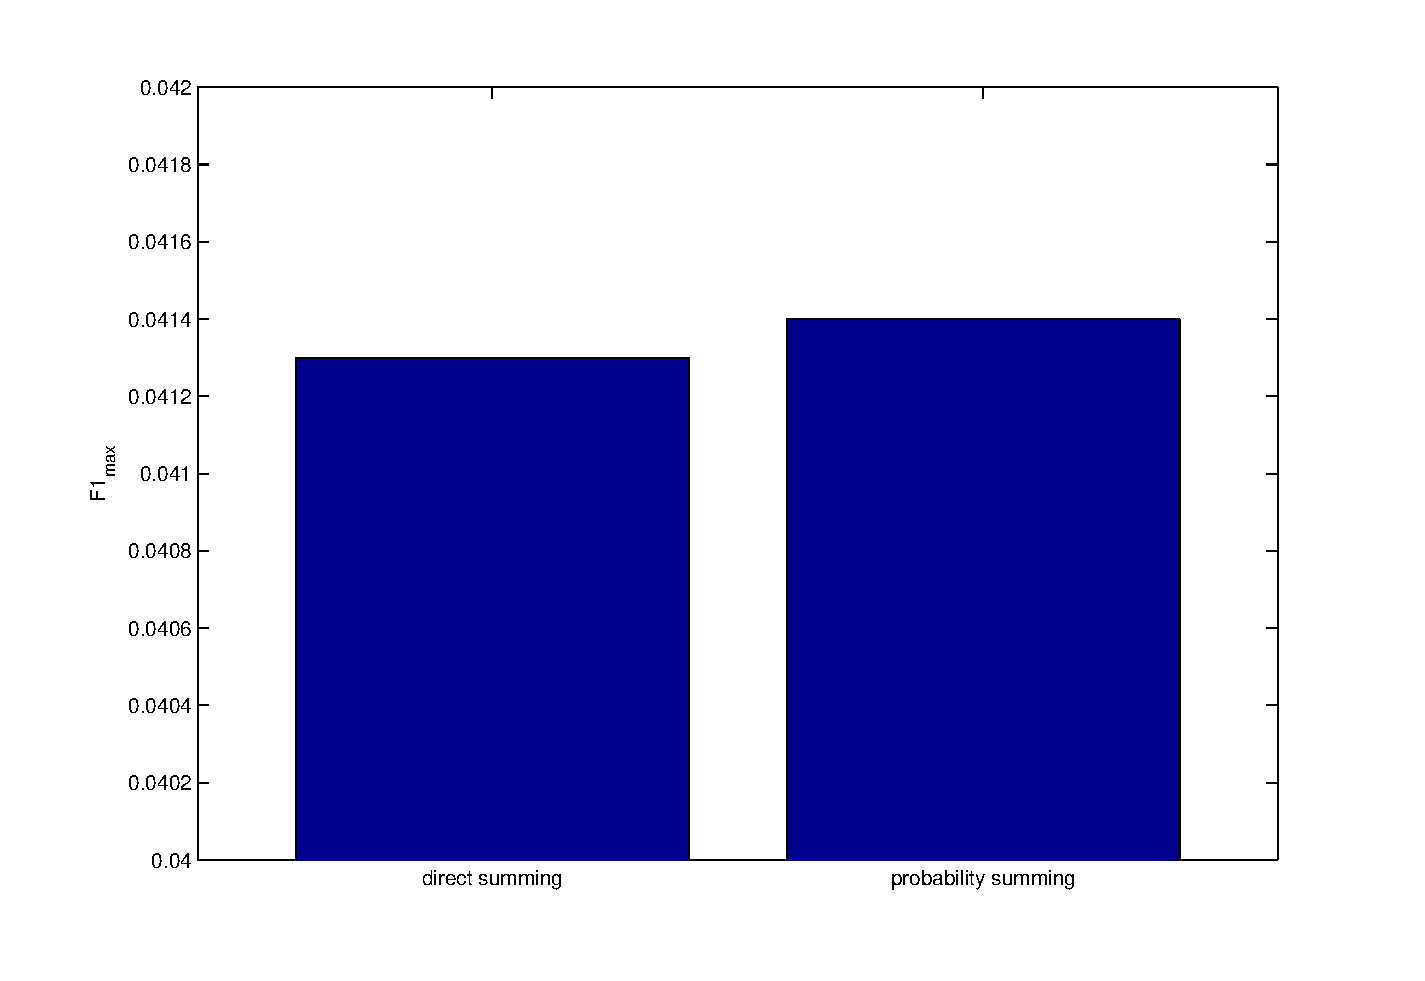
\includegraphics[width=\linewidth]{./summing_compare_f1.eps}
\end{frame}


\begin{frame}{Similarity Normalization}
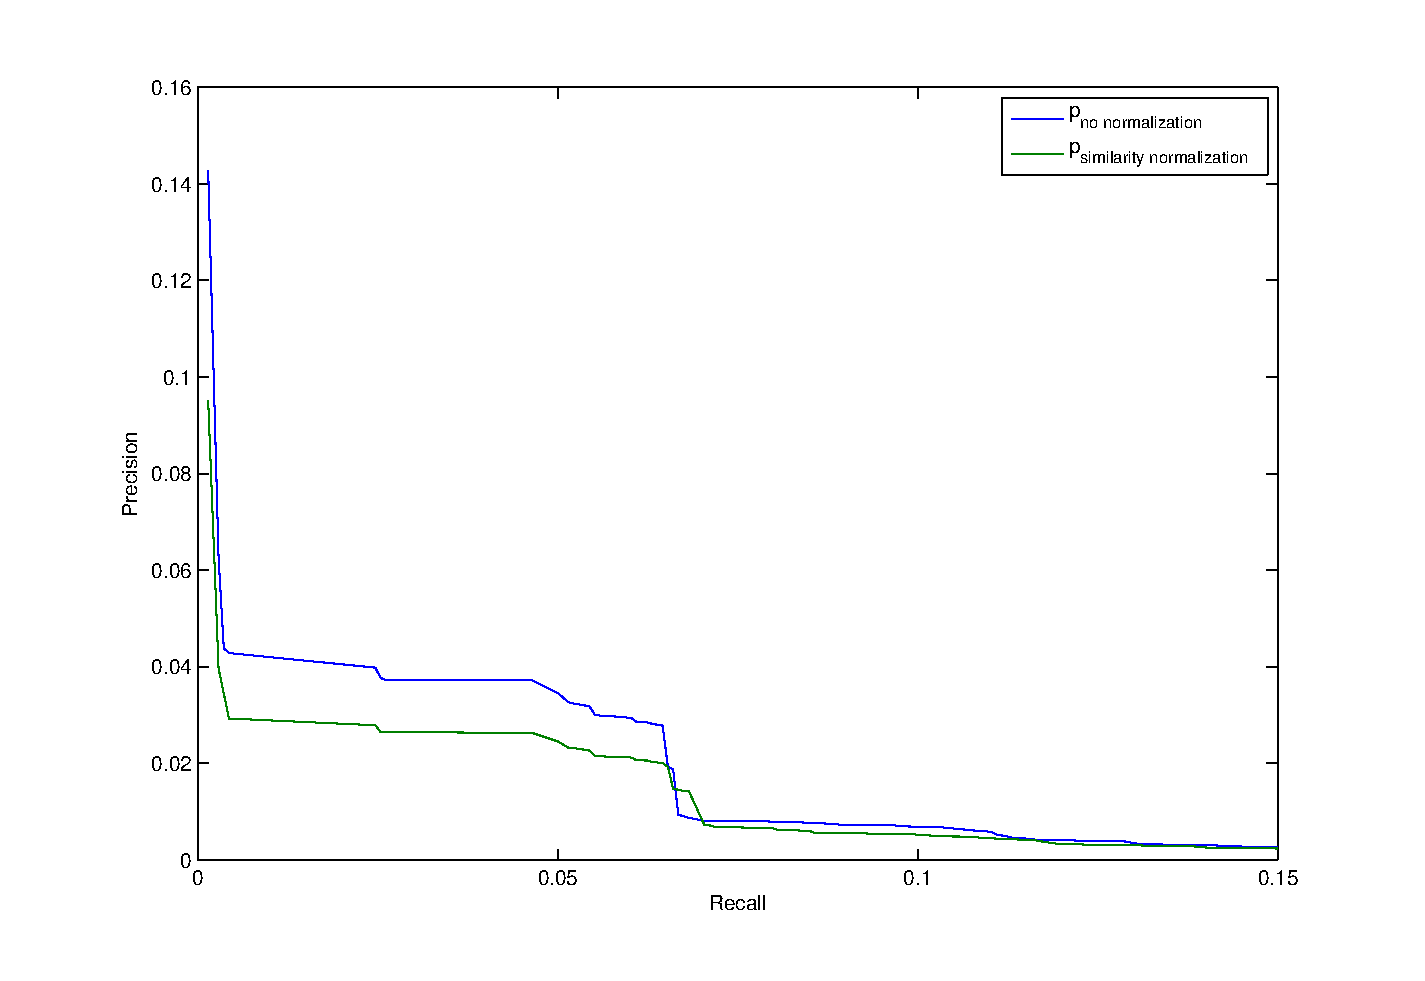
\includegraphics[width=\linewidth]{./sim_norm.eps}
\end{frame}

\begin{frame}{Similarity Normalization}
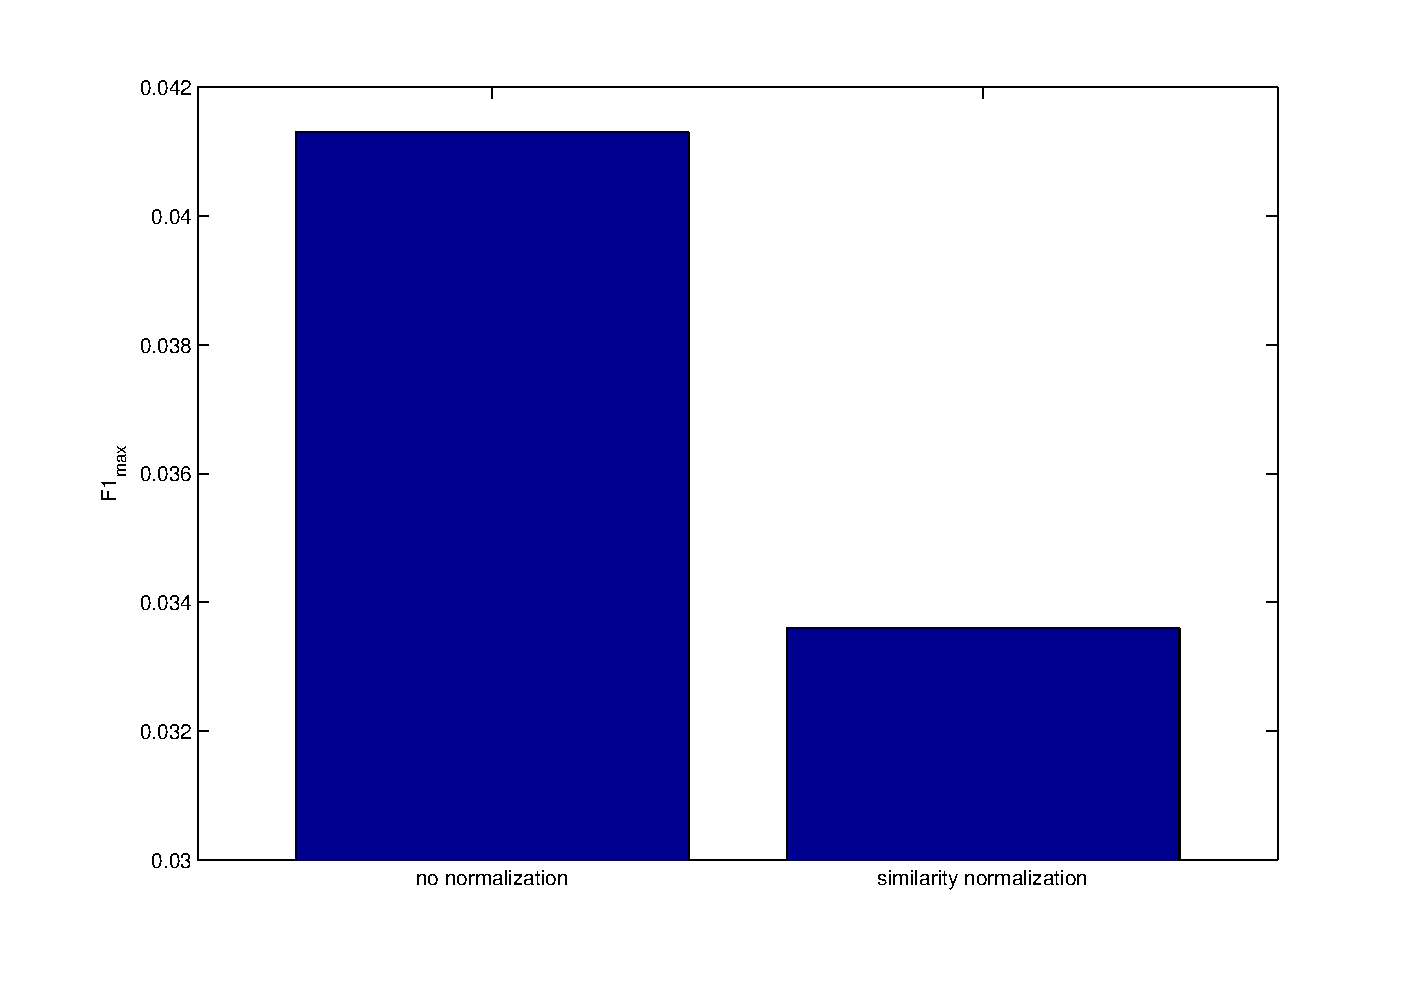
\includegraphics[width=\linewidth]{./sim_norm_f1.eps}
\end{frame}


\begin{frame}{Similarity Normalization}

\begin{itemize}
\item Dataset is so small, that many items do not have $k$ neighbors.
\item The sparse item will divide a smaller denominator, rather than larger(expected).
\end{itemize}

\end{frame}


\begin{frame}{Row Normalization}
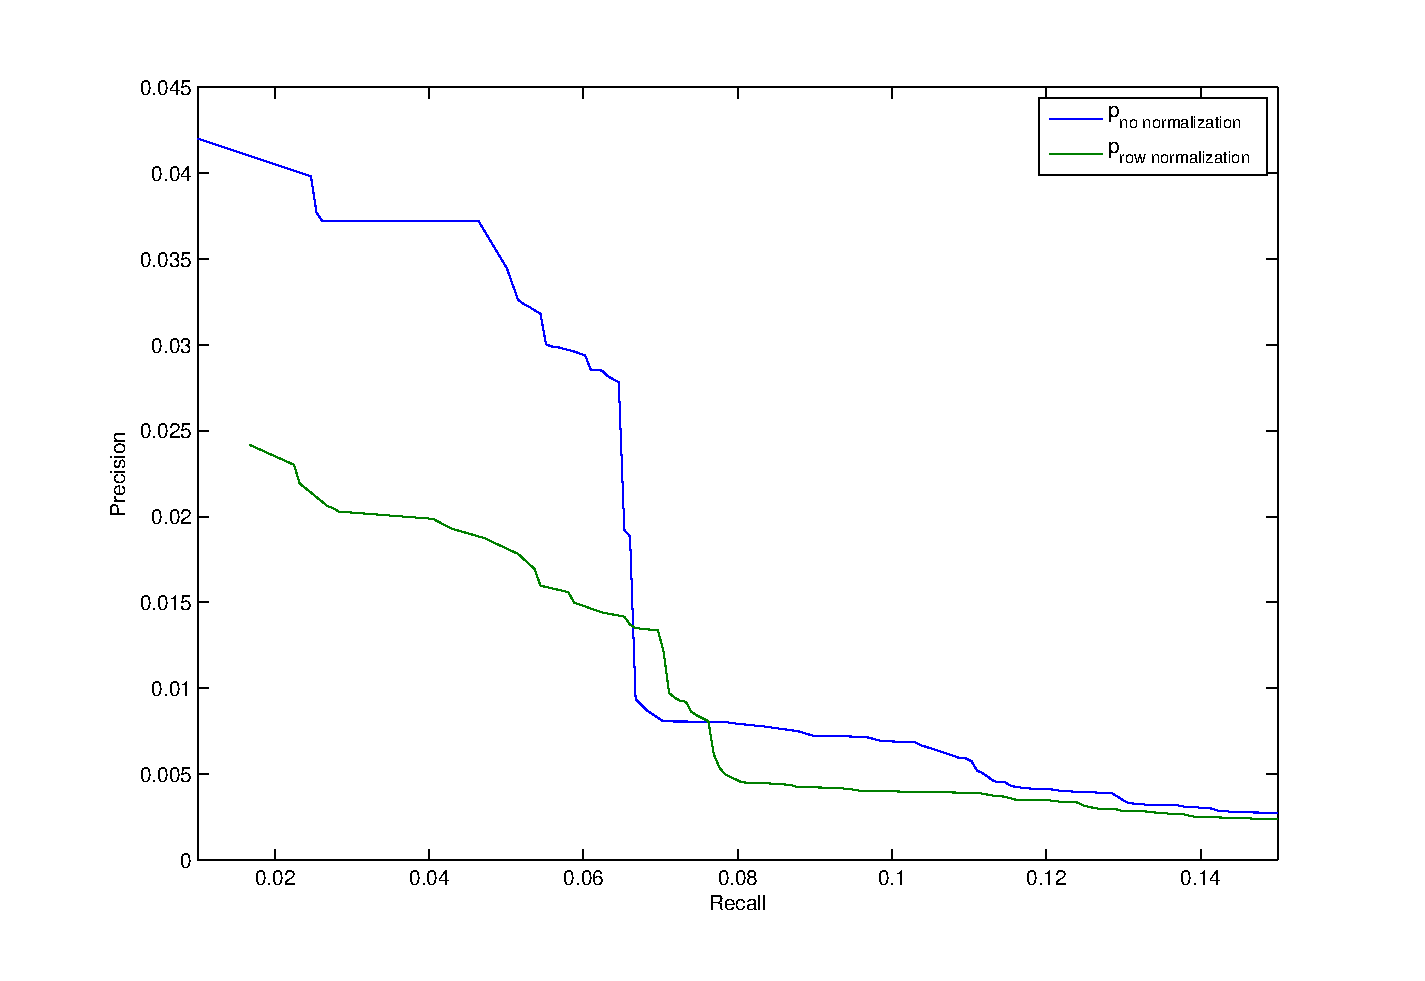
\includegraphics[width=\linewidth]{./row_norm.eps}
\end{frame}

\begin{frame}{Row Normalization}
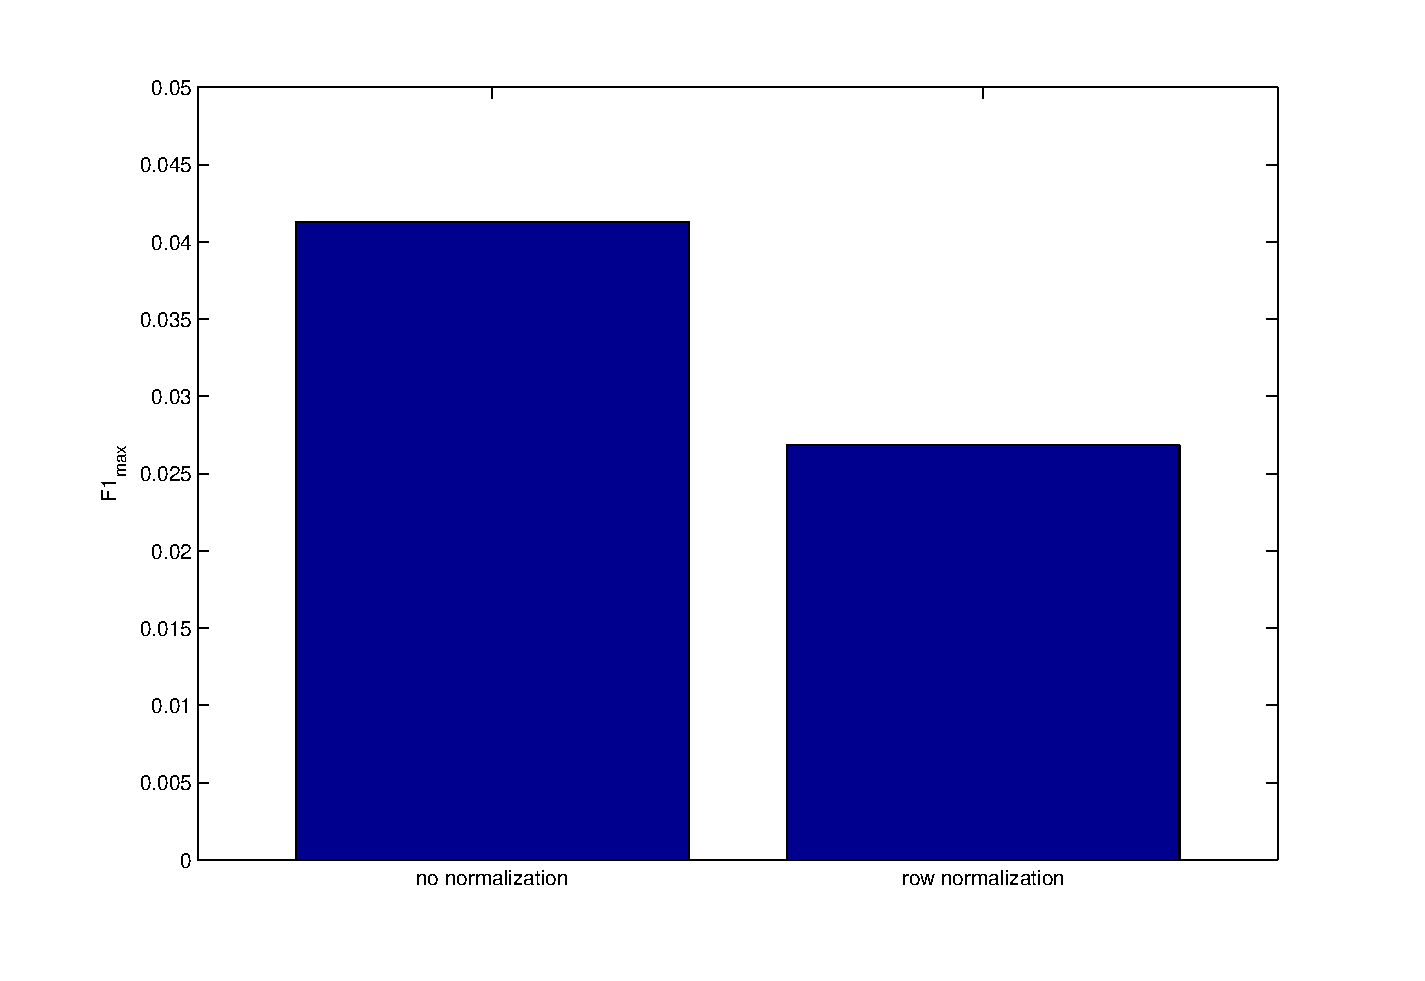
\includegraphics[width=\linewidth]{./row_norm_f1.eps}
\end{frame}


\begin{frame}{Row Normalization}

\begin{itemize}
\item Row normalization results in equal purchasing power for each user.
\item This side-effect is considerable. Users who purchase alot certainly will purchase a lot.
\end{itemize}

\begin{alertblock}{Case for Top-N Recommendation}
\begin{itemize}
\item Top-N recommendation system will recommend N item for each user.
\item Normalizing purchasing power has no side-effect.
\item Row Normalization is useful now.
\end{itemize}
\end{alertblock}

\end{frame}


\subsection{Comparison with User-based CF}

\begin{frame}{P-R Relationship}
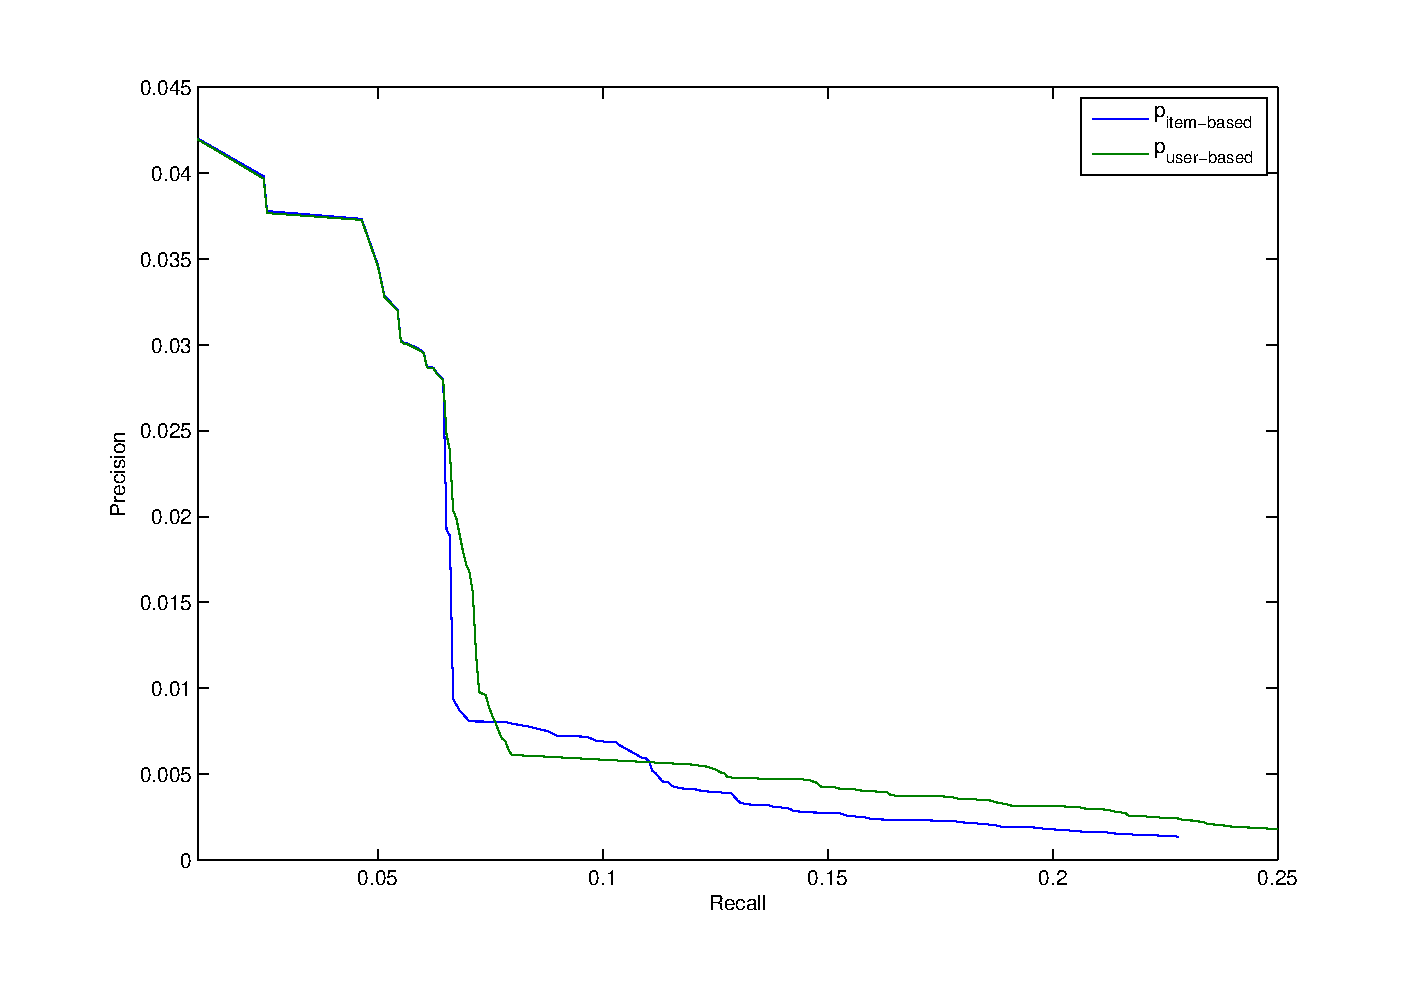
\includegraphics[width=\linewidth]{./base.eps}
\end{frame}

\begin{frame}{Max F1}
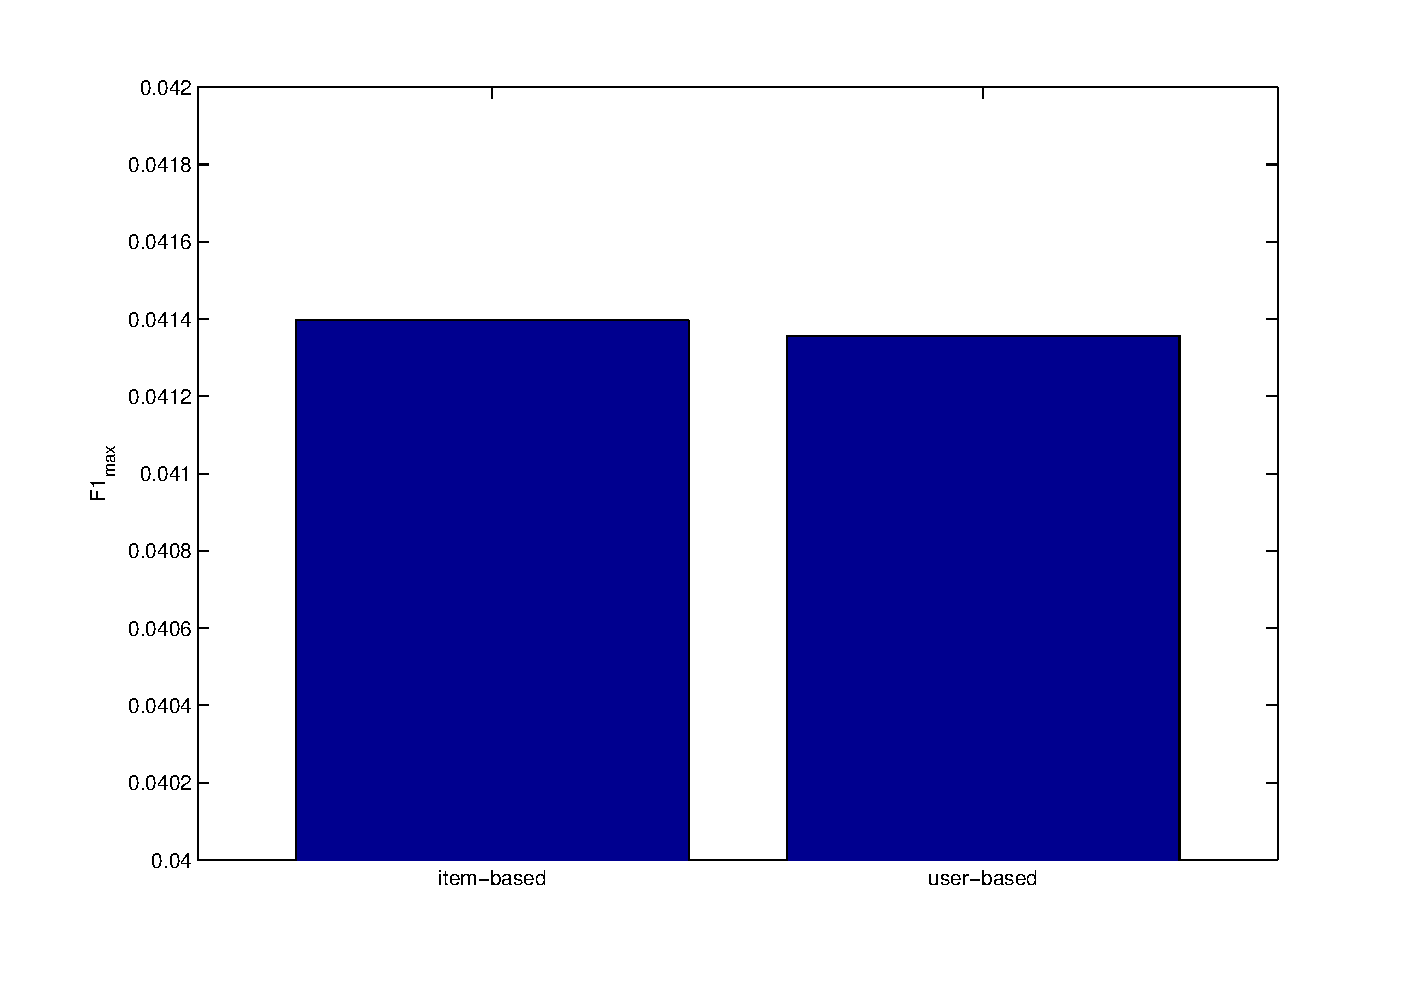
\includegraphics[width=\linewidth]{./base_f1.eps}
\end{frame}



\subsection*{Thanks}


\begin{frame}%[allowframebreaks]
\frametitle<presentation>{References}
\begin{thebibliography}{10}
\beamertemplatearticlebibitems
\bibitem{karypis2001}
Karypis G.
\newblock {\em Evaluation of item-based top-n recommendation \\ algorithms[C]}.
\newblock Proceedings of the 10th international conference on Information and knowledge management. ACM, 2001: 247-254.
\bibitem{Sarwar2001}
Sarwar B, Karypis G, Konstan J, et al.
\newblock {\em Item-based collaborative filtering recommendation algorithms[C]}.
\newblock Proceedings of the 10th international conference on World Wide Web. ACM, 2001: 285-295.
\end{thebibliography}
\end{frame}

\begin{frame}[fragile]{Thanks}
\begin{center}
{\huge Thank you!}
\end{center}
\end{frame}

%------------------------------------------End----------------------------------------------
\end{document}
